% Companion code structure and usage guide for HydrogenMSG.
% Code: https://github.com/hanfengzhai/HydrogenMSG
\documentclass[11pt]{article}
\usepackage[margin=0.75in]{geometry}
\usepackage{iftex}
\ifPDFTeX
  \usepackage[T1]{fontenc}
\fi
\usepackage{amsmath,amssymb,mathtools}
\usepackage{array}
\usepackage{tabularx}
\usepackage{booktabs}
\usepackage{placeins}
\usepackage{xcolor}
\usepackage{listings}
\usepackage{tikz}
\usetikzlibrary{arrows.meta,positioning,shapes.multipart,fit}

\definecolor{RunShellBg}{RGB}{243,247,253}
\definecolor{RunShellFrame}{RGB}{58,112,168}
\definecolor{RunPyBg}{RGB}{243,250,248}
\definecolor{RunPyFrame}{RGB}{36,126,115}
\definecolor{TermBg}{RGB}{248,248,246}
\definecolor{TermFrame}{RGB}{125,135,148}
\definecolor{CodeKw}{RGB}{0,84,179}
\definecolor{CodeStr}{RGB}{163,21,21}
\definecolor{CodeCom}{RGB}{34,126,58}
\definecolor{CodeEmph}{RGB}{118,52,168}

\lstdefinestyle{runshell}{
  language=bash,
  alsoletter={-},
  basicstyle=\ttfamily\fontsize{8.5}{10.8}\selectfont\color{black!92},
  backgroundcolor=\color{RunShellBg},
  frame=single,
  rulecolor=\color{RunShellFrame},
  framerule=0.8pt,
  xleftmargin=2pt,
  xrightmargin=2pt,
  framesep=6pt,
  breaklines=true,
  breakatwhitespace=false,
  columns=fixed,
  basewidth=0.50em,
  keepspaces=true,
  aboveskip=6pt,
  belowskip=8pt,
  showstringspaces=false,
  keywordstyle=\color{CodeKw}\bfseries,
  commentstyle=\color{CodeCom}\itshape,
  stringstyle=\color{CodeStr},
  emphstyle=\color{CodeEmph}\bfseries,
  morekeywords={git,clone,cd,python3,pip,install,hydrogenmsg-figures},
  emph={--list,--manuscript,-m,-e,-r,-c}
}

\lstdefinestyle{runpython}{
  language=Python,
  basicstyle=\ttfamily\fontsize{8.5}{10.8}\selectfont\color{black!92},
  backgroundcolor=\color{RunPyBg},
  frame=single,
  rulecolor=\color{RunPyFrame},
  framerule=0.8pt,
  xleftmargin=2pt,
  xrightmargin=2pt,
  framesep=6pt,
  breaklines=true,
  breakatwhitespace=false,
  columns=fixed,
  basewidth=0.50em,
  keepspaces=true,
  aboveskip=6pt,
  belowskip=8pt,
  showstringspaces=false,
  keywordstyle=\color{CodeKw}\bfseries,
  commentstyle=\color{CodeCom}\itshape,
  stringstyle=\color{CodeStr},
  emphstyle=\color{CodeEmph}\bfseries,
  emph={Params,torsion_Q,bending_average_uptake,void_fields,cavitation_stress}
}

\lstdefinestyle{termout}{
  basicstyle=\ttfamily\fontsize{7.9}{9.9}\selectfont\color{black!90},
  backgroundcolor=\color{TermBg},
  frame=single,
  rulecolor=\color{TermFrame},
  framerule=0.7pt,
  xleftmargin=2pt,
  xrightmargin=2pt,
  framesep=5.5pt,
  breaklines=true,
  breakatwhitespace=false,
  columns=fixed,
  basewidth=0.44em,
  keepspaces=true,
  aboveskip=5pt,
  belowskip=7pt,
  showstringspaces=false,
  comment=[l]{\#},
  commentstyle=\color{CodeCom}\bfseries,
  emphstyle=\color{CodeKw}\bfseries,
  emph={torsion,bending,HELP}
}
\usepackage[colorlinks=true,linkcolor=blue!60!black,citecolor=blue!60!black,urlcolor=blue!60!black]{hyperref}
\usepackage{setspace}
\setstretch{1.02}
\renewcommand{\topfraction}{0.92}
\renewcommand{\bottomfraction}{0.90}
\renewcommand{\textfraction}{0.06}
\renewcommand{\floatpagefraction}{0.78}

\title{\textbf{HydrogenMSG: Code Architecture, Prerequisites, and Usage Guide}}
\author{Hanfeng Zhai}
\date{}

\begin{document}
\maketitle

\begin{abstract}
\texttt{HydrogenMSG} provides the Python analytical library, two-dimensional finite-element solvers, and figure generation pipeline accompanying the study of size-dependent hydrogen transport and trapping in mechanism-based strain gradient (MSG) plasticity.
%
This guide summarizes the software prerequisites, layered package architecture, command-line workflows, verified outputs, and interactive browser companion tool so every calculation and manuscript figure can be reproduced cleanly.
\end{abstract}

\section{Overview and Interactive Browser GUI}

The public repository at \url{https://github.com/hanfengzhai/HydrogenMSG} organizes the codebase into three layers under \texttt{hydrogenmsg/}: closed-form MSG--Oriani solutions (\texttt{analytics}), lower-order Q9 finite-element checks (\texttt{fem}), and figure builders (\texttt{plot}).
%
For interactive parameter exploration without installing Python locally, a browser GUI application is hosted online at:
\begin{quote}
\centering
\url{https://hanfengzhai.github.io/HydrogenMSG.html}
\end{quote}
Users exploring parameter sensitivities for torsion, bending, spherical void trapping, or HELP cavitation can use the browser interface directly; local installation is needed only to call the Python API, run finite-element checks, or regenerate figure files.

\section{Prerequisites and Installation}

\texttt{HydrogenMSG} depends only on a lightweight scientific Python stack with no external compiled FEM solvers or platform-specific extensions (Table~\ref{tab:prereqs}).

\begin{table}[!htbp]
\centering
\caption{Software prerequisites declared in \texttt{pyproject.toml} and \texttt{requirements.txt}.}
\label{tab:prereqs}
\small
\setlength{\tabcolsep}{6pt}
\begin{tabularx}{\textwidth}{@{}>{\raggedright\arraybackslash}l >{\raggedright\arraybackslash}l >{\raggedright\arraybackslash}X@{}}
\toprule
Component & Requirement & Role in \texttt{HydrogenMSG} \\
\midrule
Python & $\ge 3.10$ & Dataclasses, union type annotations, \texttt{argparse} CLI \\
NumPy & $\ge 1.24$ & Array kinematics, constitutive laws, Gauss integration \\
SciPy & $\ge 1.10$ & Sparse Q9 assembly and LU solves (\texttt{coo\_matrix}, \texttt{spsolve}, \texttt{splu}) \\
Matplotlib & $\ge 3.7$ & Vector PDF and $200$\,DPI PNG rendering in \texttt{hydrogenmsg.plot} \\
Build backend & \texttt{setuptools} $\ge 61$ & Editable install and \texttt{hydrogenmsg-figures} entry point \\
\bottomrule
\end{tabularx}
\end{table}

\noindent\begin{minipage}{\textwidth}
\begin{lstlisting}[style=runshell]
# 1. Clone the public repository
git clone https://github.com/hanfengzhai/HydrogenMSG.git && cd HydrogenMSG

# 2. Install runtime dependencies and editable package (recommended)
python3 -m pip install -r requirements.txt
python3 -m pip install -e .

# 3. Verify package import and console entry point
python3 -c "from hydrogenmsg import Params; p = Params(); print(f'l = {p.l*1e6:.2f} um')"
hydrogenmsg-figures --list
\end{lstlisting}
\end{minipage}

\section{Repository and Package Structure}

Dependencies flow strictly downward from constitutive closures in \texttt{analytics.py} to \texttt{fem/} and \texttt{plot/} (Figure~\ref{fig:code_arch} and Table~\ref{tab:modules}).

\begin{figure}[!htbp]
\centering
\resizebox{\textwidth}{!}{%
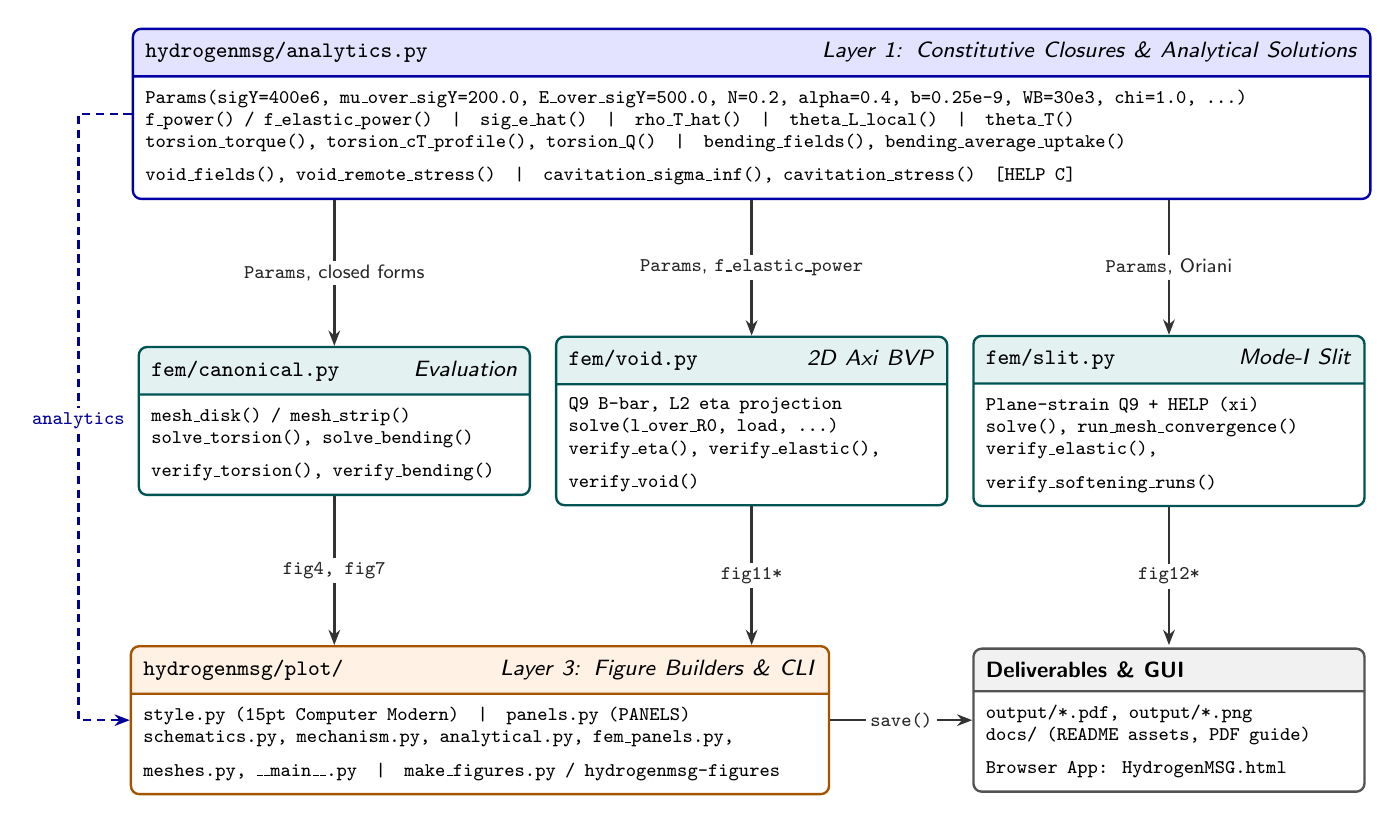
\begin{tikzpicture}[
  font=\sffamily,
  codecard/.style 2 args={
    rectangle split,
    rectangle split parts=2,
    rectangle split part fill={#1!11, white},
    rectangle split draw splits=true,
    draw=#1!65!black,
    rounded corners=3pt,
    line width=0.85pt,
    align=left,
    inner sep=4.5pt,
    text width=#2
  },
  arr/.style={-{Stealth[length=5.5pt,width=4.2pt]}, line width=0.95pt, draw=black!80},
  darr/.style={-{Stealth[length=5.5pt,width=4.2pt]}, line width=0.85pt, densely dashed, draw=blue!60!black},
  lbl/.style={font=\scriptsize\sffamily, fill=white, inner sep=1.6pt, text=black!85}
]

% Tier 1: Core theory library
\node[codecard={blue}{15.4cm}] (analytics) at (8.1, 9.6) {%
  {\footnotesize\textbf{\texttt{hydrogenmsg/analytics.py}}\hfill\textit{Layer 1: Constitutive Closures \& Analytical Solutions}}%
  \nodepart{second}%
  {\scriptsize\ttfamily
  Params(sigY=400e6, mu\_over\_sigY=200.0, E\_over\_sigY=500.0, N=0.2, alpha=0.4, b=0.25e-9, WB=30e3, chi=1.0, ...)\\
  f\_power() / f\_elastic\_power() \ | \ sig\_e\_hat() \ | \ rho\_T\_hat() \ | \ theta\_L\_local() \ | \ theta\_T()\\
  torsion\_torque(), torsion\_cT\_profile(), torsion\_Q() \ | \ bending\_fields(), bending\_average\_uptake()\\
  void\_fields(), void\_remote\_stress() \ | \ cavitation\_sigma\_inf(), cavitation\_stress() \ [HELP C]
  }%
};

% Tier 2: FEM modules
\node[codecard={teal}{4.65cm}] (canonical) at (2.8, 5.7) {%
  {\footnotesize\textbf{\texttt{fem/canonical.py}}\hfill\textit{Evaluation}}%
  \nodepart{second}%
  {\scriptsize\ttfamily
  mesh\_disk() / mesh\_strip()\\
  solve\_torsion(), solve\_bending()\\
  verify\_torsion(), verify\_bending()
  }%
};

\node[codecard={teal}{4.65cm}] (void) at (8.1, 5.7) {%
  {\footnotesize\textbf{\texttt{fem/void.py}}\hfill\textit{2D Axi BVP}}%
  \nodepart{second}%
  {\scriptsize\ttfamily
  Q9 B-bar, L2 eta projection\\
  solve(l\_over\_R0, load, ...)\\
  verify\_eta(), verify\_elastic(),\\
  verify\_void()
  }%
};

\node[codecard={teal}{4.65cm}] (slit) at (13.4, 5.7) {%
  {\footnotesize\textbf{\texttt{fem/slit.py}}\hfill\textit{Mode-I Slit}}%
  \nodepart{second}%
  {\scriptsize\ttfamily
  Plane-strain Q9 + HELP (xi)\\
  solve(), run\_mesh\_convergence()\\
  verify\_elastic(),\\
  verify\_softening\_runs()
  }%
};

% Tier 3: Plotting package & CLI (wider gap before Deliverables so save() sits cleanly on arrow)
\node[codecard={orange}{8.55cm}] (plot) at (4.65, 1.9) {%
  {\footnotesize\textbf{\texttt{hydrogenmsg/plot/}}\hfill\textit{Layer 3: Figure Builders \& CLI}}%
  \nodepart{second}%
  {\scriptsize\ttfamily
  style.py (15pt Computer Modern) \ | \ panels.py (PANELS)\\
  schematics.py, mechanism.py, analytical.py, fem\_panels.py,\\
  meshes.py, \_\_main\_\_.py \ | \ make\_figures.py / hydrogenmsg-figures
  }%
};

\node[codecard={gray}{4.65cm}] (outputs) at (13.4, 1.9) {%
  {\footnotesize\textbf{Deliverables \& GUI}}%
  \nodepart{second}%
  {\scriptsize\ttfamily
  output/*.pdf, output/*.png\\
  docs/ (README assets, PDF guide)\\
  Browser App: HydrogenMSG.html
  }%
};

% Clean orthogonal routing
\draw[arr] (analytics.south -| canonical.north) -- (canonical.north) node[lbl, midway] {\texttt{Params}, closed forms};
\draw[arr] (analytics.south) -- (void.north) node[lbl, midway] {\texttt{Params}, \texttt{f\_elastic\_power}};
\draw[arr] (analytics.south -| slit.north) -- (slit.north) node[lbl, midway] {\texttt{Params}, Oriani};

\draw[arr] (canonical.south) -- (canonical.south |- plot.north) node[lbl, midway] {\texttt{fig4, fig7}};
\draw[arr] (void.south) -- (void.south |- plot.north) node[lbl, midway] {\texttt{fig11*}};
\draw[arr] (slit.south) -- (slit.south |- plot.north) node[lbl, midway] {\texttt{fig12*}};
\draw[darr] (analytics.west) -- (-0.45, 9.6) -- (-0.45, 1.9) -- (plot.west);
\node[lbl, text=blue!60!black] at (-0.45, 5.7) {\texttt{analytics}};

\draw[arr] (plot.east) -- (outputs.west) node[lbl, midway] {\texttt{save()}};
\end{tikzpicture}%
}
\caption{Layered architecture of \texttt{HydrogenMSG}. Unidirectional dataflow passes parameters and analytical closures from \texttt{analytics.py} into the finite-element solvers (\texttt{fem/}) and unified plotting modules (\texttt{plot/}).}
\label{fig:code_arch}
\end{figure}
\FloatBarrier

\begin{table}[!htbp]
\centering
\caption{Directory and module map of the \texttt{HydrogenMSG} repository.}
\label{tab:modules}
\footnotesize
\setlength{\tabcolsep}{5pt}
\begin{tabularx}{\textwidth}{@{}>{\raggedright\arraybackslash}l >{\raggedright\arraybackslash}l >{\raggedright\arraybackslash}X@{}}
\toprule
Path & Layer & Responsibility \\
\midrule
\texttt{pyproject.toml}, \texttt{requirements.txt} & Packaging & Package metadata, minimum versions, and \texttt{hydrogenmsg-figures} CLI \\
\texttt{make\_figures.py} & CLI wrapper & Thin top-level launcher forwarding directly to \texttt{hydrogenmsg.plot.\_\_main\_\_} \\
\texttt{hydrogenmsg/\_\_init\_\_.py} & Facade & Re-exports \texttt{Params} at package root \\
\texttt{hydrogenmsg/analytics.py} & Theory & Closed-form torsion, bending, void, Oriani, and HELP cavitation solvers \\
\texttt{hydrogenmsg/fem/canonical.py} & FEM eval. & Q9 mesh evaluation checking analytical torsion and bending profiles \\
\texttt{hydrogenmsg/fem/void.py} & FEM BVP & Axisymmetric 9-node B-bar solver with covariant $L^2$ strain-gradient projection \\
\texttt{hydrogenmsg/fem/slit.py} & FEM BVP & Plane-strain mode-I slit Q9 solver with optional HELP softening (\texttt{Params.xi}) \\
\texttt{hydrogenmsg/plot/style.py} & Plotting & Shared $15$\,pt Computer Modern style and PDF + $200$\,DPI PNG exporter \\
\texttt{hydrogenmsg/plot/panels.py} & Registry & Maps panel names to builders (\texttt{DEFAULT\_ORDER}, \texttt{MANUSCRIPT\_ORDER}) \\
\texttt{hydrogenmsg/plot/\{schematics,mechanism\}.py} & Figures & Conceptual diagrams (\texttt{fig\_mechanism}, \texttt{fig1*}, \texttt{fig2*}, \texttt{fig5*}, \texttt{fig8*}) \\
\texttt{hydrogenmsg/plot/analytical.py} & Figures & Analytical curves and profiles (\texttt{fig3*}, \texttt{fig6*}, \texttt{fig9*}, \texttt{fig10*}) \\
\texttt{hydrogenmsg/plot/\{fem\_panels,meshes\}.py} & Figures & FEM result panels (\texttt{fig4*}, \texttt{fig7*}, \texttt{fig11*}, \texttt{fig12*}) and mesh views \\
\texttt{output/}, \texttt{docs/} & Assets & Generated PDF/PNG output folder (gitignored) and README/documentation assets \\
\bottomrule
\end{tabularx}
\end{table}
\FloatBarrier

\section{Reproducible Execution Workflows}

\subsection{Using the Theory Library}

All analytical models operate on the \texttt{Params} dataclass, whose defaults follow bcc iron hydrogen parameters and Huang-style MSG constants ($\sigma_{\mathrm{Y}}=400\,\mathrm{MPa}$, $\mu/\sigma_{\mathrm{Y}}=200$, $E/\sigma_{\mathrm{Y}}=500$, $l=4.80\,\mu\mathrm{m}$, $W_{\mathrm{B}}=30\,\mathrm{kJ/mol}$).

\noindent\begin{minipage}{\textwidth}
\begin{lstlisting}[style=runpython]
from hydrogenmsg import Params
from hydrogenmsg.analytics import (
    torsion_Q, bending_average_uptake, void_fields, cavitation_stress
)

p = Params()                                    # default MSG + bcc-iron hydrogen constants
Q = torsion_Q(a=1e-6, Gamma=0.05, p=p)          # torsion uptake enhancement Q(a)
cL_avg, cT_avg = bending_average_uptake(h=1e-6, eps_s=0.05, p=p)
p_help = Params(thetaL0=1e-5, xi=0.3)           # Formulation C HELP cavitation
sig_c = cavitation_stress(l_over_R0=10.0, p=p_help)
print(f"l = {p.l*1e6:.2f} um | Q(1 um) = {Q:.4f} | cT_avg = {cT_avg:.4f} | sig_c/sigY = {sig_c:.3f}")
# -> l = 4.80 um | Q(1 um) = 1.0990 | cT_avg = 3.3368 | sig_c/sigY = 6.577
\end{lstlisting}
\end{minipage}

\subsection{Reproducing Manuscript and Companion Figures}

Every figure is registered under \texttt{hydrogenmsg.plot.panels.PANELS} and writes both vector \texttt{.pdf} and raster \texttt{.png} files into \texttt{output/}.
%
Schematics and analytical curves run in a few seconds; the mode-I slit panels (\texttt{fig12*}) solve fine $80\times 40$ tip-window nonlinear problems and take longer on a single CPU core.

\noindent\begin{minipage}{\textwidth}
\begin{lstlisting}[style=runshell]
# List all 27 manuscript panels and 20 companion panels
python3 -m hydrogenmsg.plot --list

# Build only panels cited in the manuscript LaTeX source (writes to output/)
python3 make_figures.py --manuscript
# Or use the installed console entry point: hydrogenmsg-figures --manuscript

# Build individual panels or FEM mesh visualizations on demand
python3 -m hydrogenmsg.plot fig3b fig6d fig10a
python3 -m hydrogenmsg.plot.meshes
python3 -m hydrogenmsg.plot                      # full suite (including SI + fig12* slit solves)
\end{lstlisting}
\end{minipage}

\subsection{Running Finite-Element Verification Checks}

Each module in \texttt{hydrogenmsg.fem} provides an executable \texttt{\_\_main\_\_} verification suite checking discretization and boundary-value accuracy against the analytical solutions.

\noindent\begin{minipage}{\textwidth}
\begin{lstlisting}[style=runshell]
# 1. Canonical torsion & bending Q9 evaluations against closed forms
python3 -m hydrogenmsg.fem.canonical

# 2. Axisymmetric void B-bar FEM: strain-gradient operator, Lame elastic limit, plastic zone R<=2 R0
python3 -m hydrogenmsg.fem.void

# 3. Plane-strain mode-I slit kinematics, elastic near-tip check, and HELP softening demo
python3 -m hydrogenmsg.fem.slit
\end{lstlisting}
\end{minipage}

\medskip
\noindent\textbf{Verified output.}
Running the three commands above produces the terminal output below:

\noindent\begin{minipage}{\textwidth}
\begin{lstlisting}[style=termout]
# python3 -m hydrogenmsg.fem.canonical
torsion: {'cT_err': 4.714071409068731e-16, 'T_fem': 1.9247552442625562, 'T_an': 1.9713459654999823, 'T_rel': 0.023633964840671484}
bending: {'sig_m_err': 2.220446049250313e-16, 'cT_err': 5.254566250143749e-16}

# python3 -m hydrogenmsg.fem.void
strain-gradient operator vs 3 sqrt(5/2) A/R^4:  median 0.79%, max 0.86%
elastic limit vs Lame cavity solution:  sigma_m 0.00%, sigma_e 0.09%, u0 0.03%
plastic fields vs closed form, l/R0 = 0.0 (delta = 0.0098, R <= 2 R0):  eps_e 0.05%, sigma_e 0.01%, sigma_m 2.10%
plastic fields vs closed form, l/R0 = 1.0 (delta = 0.0098, R <= 2 R0):  eps_e 0.05%, l*eta 1.00%, sigma_e 0.01%, sigma_m 2.09%
plastic fields vs closed form, l/R0 = 5.0 (delta = 0.0095, R <= 2 R0):  eps_e 0.05%, l*eta 1.01%, sigma_e 0.04%, sigma_m 2.06%

# python3 -m hydrogenmsg.fem.slit
mesh + kinematics smoke ...
  nodes 5313, elems 1292, tip at (1.000, 0.000)
elastic near-tip sigma_yy vs K_I/sqrt(2 pi r):  median 17.0%, max 27.2%, COD/a=1.5024e-04, iters=8
HELP softening demo:  iters=306, resid=3.89e-08, COD/a=4.4914e-03, soft in [0.913, 1], mean 0.951, max eps_e=0.0286, max sig_e/sigY=3.093
\end{lstlisting}
\end{minipage}

\end{document}
